\documentclass{article}

\usepackage{graphicx}
\usepackage{subcaption}
\usepackage{amsmath, amssymb}
\usepackage{bm}
\usepackage{appendix}
\usepackage{float}
\usepackage{tabularx}
\usepackage{tikz}
\usepackage[section]{placeins}
\usepackage{listings}

\begin{document}

\title{\vspace{1cm}Project 4 \\ FYS3150}

\author{\vspace{1cm}Ann-Silje Kirkvik \\ github.com/annsilje/fys3150}
\date{\vspace{5cm}\today}

\maketitle

\newpage

\begin{abstract}
This project studies the Ising model in two dimension to simulate a second order phase transition in a magnetic system as the temperature increases. The system is modeled as a square lattice of grid points with spin up or down. The Metropolis algorithm is used to run this simulation. First, a simple $2\times 2$ lattice is tested to verify that the numerical solution agrees with the analytical solution. Then, a larger lattice ($20 \times 20$) is tested to investigate the behavior of the expectation values during the Monte Carlo cycles. The tests indicate that at least $10^6$ Monte Carlo cycles is needed to reach a steady state. Finally, multiple lattices are simulated where the temperature is gradually increased towards and beyond the critical temperature. With $10^6$ Monte Carlo cycles the critical temperature is correct with respect to the theoretical solution up to 3 digits. The Metropolis algorithm is computational heavy since many Monte Carlo cycles are needed, but the algorithm is fairly easy to parallelize and it benefits greatly from both optimization and parallelization.
\end{abstract}

\vspace{1cm}


\section{Introduction}
This project studies the Ising model in two dimension to simulate a second order phase transition in a magnetic system as the temperature increases. The system is modeled as a square lattice of grid points with spin up or down. The analytical solution for a $2\times 2$ lattice is calculated, but for larger lattices numerical methods are needed. This project utilizes the Metropolis algorithm and can then simulate the behavior of the system as the temperature increases. Section \ref{sec:description} describes the theoretical background of the project and the implementation. Section \ref{sec:results} shows the results of the numerical experiments and section \ref{sec:conclusions} has some final remarks.


\section{Description}
\label{sec:description}
This project studies the Ising model in two dimension to simulate a second order phase transition in a magnetic system as the temperature increases. The system is modeled as a two dimensional square lattice where each grid point has a spin that is either up or down. At low temperatures this system will have a net magnetization different from zero, but when the system reaches the critical temperature, $T_C$, where the phase transition occurs, the net magnetization becomes zero. The energy of the system in this model is

\begin{equation}
E = - J \sum\limits_{<kl>}^N s_ks_l - \mathcal{B} \sum\limits_{k=1}^N s_k
\label{eq:energy}
\end{equation}

\noindent where $s_k$ is the spin with value $\pm1$, $N=L\times L$ is the number of spins in the lattice of size $L$, $J$ is a coupling constant that says something about the strength of the interactions and is in this project assumed to be positive. $\mathcal{B}$ is the external magnetic field, but in this project there will be no external magnetic field which means $\mathcal{B}=0$. $<kl>$ is the sum over nearest neighbors. The magnetization of the system is given by

\begin{equation}
\mathcal{M} = \sum\limits_{i=1}^N s_i
\label{eq:magnetization}
\end{equation}

\begin{figure}
\centering
\subcaptionbox{Free ends\label{subfig:fe}}[0.45\textwidth]{%
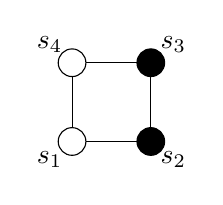
\begin{tikzpicture}
    \draw (0,0) -- (0,1);
    \draw (0,0) -- (1,0);
    \draw (1,1) -- (1,0);
    \draw (1,1) -- (0,1);

    \draw[fill=white](0,0) circle (5pt);
    \draw[fill=white](0,1) circle (5pt);
    \filldraw (1,0) circle (5pt);
    \filldraw (1,1) circle (5pt);
    
    \node [below left] at (0,0) {$s_1$};
    \node [below right] at (1,0) {$s_2$};
    \node [above left] at (0,1) {$s_4$};
    \node [above right] at (1,1) {$s_3$};
\end{tikzpicture}
}
\subcaptionbox{Periodic boundary conditions\label{subfig:pbc}}[0.45\textwidth]{%
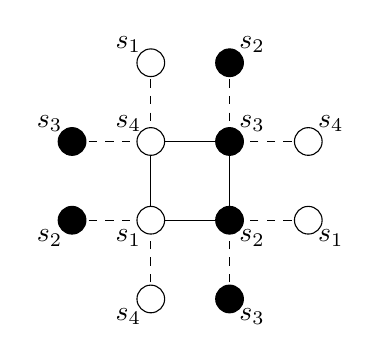
\begin{tikzpicture}
    \draw (0,0) -- (0,1);
    \draw (0,0) -- (1,0);
    \draw (1,1) -- (1,0);
    \draw (1,1) -- (0,1);
    \draw [dashed](-1,0) -- (0,0);
    \draw [dashed](0,-1) -- (0,0);
    \draw [dashed](-1,1) -- (0,1);
    \draw [dashed](0,2) -- (0,1);
    \draw [dashed](2,0) -- (1,0);
    \draw [dashed](1,-1) -- (1,0);
    \draw [dashed](1,2) -- (1,1);
    \draw [dashed](2,1) -- (1,1);

    \draw[fill=white] (0,0) circle (5pt);
    \draw[fill=white] (0,1) circle (5pt);
    \filldraw (1,0) circle (5pt);
    \filldraw (1,1) circle (5pt);
    
    \draw[fill=white] (0,2) circle (5pt);
    \draw[fill=white] (0,-1) circle (5pt);
    \draw[fill=white] (2,0) circle (5pt);
    \draw[fill=white] (2,1) circle (5pt);
    \filldraw (-1,0) circle (5pt);
    \filldraw (-1,1) circle (5pt);
    \filldraw (1,-1) circle (5pt);
    \filldraw (1,2) circle (5pt);
              
    \node [below left] at (0,0) {$s_1$};
    \node [below right] at (1,0) {$s_2$};
    \node [above left] at (0,1) {$s_4$};
    \node [above right] at (1,1) {$s_3$};

    \node [above left] at (0,2) {$s_1$};
    \node [below right] at (2,0) {$s_1$};
    \node [below left] at (-1,0) {$s_2$};
    \node [above right] at (1,2) {$s_2$};
    \node [above left] at (-1,1) {$s_3$};
    \node [below right] at (1,-1) {$s_3$};
    \node [below left] at (0,-1) {$s_4$};
    \node [above right] at (2,1) {$s_4$};
\end{tikzpicture}
}
\caption{$2\times2$ lattice of spins with different boundary conditions. White dots represent $s_k=1$ and black dots represent $s_k=-1$.}
\label{fig:2by2}
\end{figure}

Because the lattice is finite, the boundaries has to be considered specifically. Two popular approaches are free ends and periodic boundary conditions. With free ends a spin on the boundary will only have two or three neighbors as opposed to all the internal spins which have four neighbors. Free ends is illustrated in figure \ref{subfig:fe}. With periodic boundary conditions all spins have four neighbors, and the lattice wraps around at the ends such that the boundary spins have the spin on the opposite boundary as one of their neighbors, as shown in figure \ref{subfig:pbc}.

Since each spin has two legal values the lattice have a total of $M=2^N$ possible micro states. For a $2\times 2$ lattice the total number of possible micro states is 16. 

Simulating a system that exchange heat and thereby energy with its surroundings the state of the system can be represented by the canonical ensemble. In the canonical ensemble the potential function is Helmholtz' free energy, $F$, given by

\begin{equation}
F = \langle E \rangle - TS
\label{eq:free_energy}
\end{equation}

\noindent where $\langle E \rangle$ is the expectation value of the system's energy, $T$ is the temperature of the system and $S$ is the entropy of the system. The equilibrium for this potential function is compromise a between minimizing the energy of the system and maximizing the entropy. 

In the canonical ensemble the probability distribution for the system's energy is given by the Boltzmann distribution

\begin{equation}
P(\beta) = \frac{e^{-\beta E_i}}{Z}
\label{eq:boltzmann}
\end{equation}

\noindent where $\beta=1/(k_BT)$, $k_B$ is the Boltzmann constant and $T$ is the temperature. The partition function $Z$ is given by

\begin{equation}
Z = \sum\limits_{i=1}^M e^{-\beta E_i}
\label{eq:partition}
\end{equation}

\noindent The expectation values for the energy can then be calculated as 

\begin{equation}
\left\langle E \right\rangle = \sum\limits_{i=1}^M E_iP(\beta) = \frac{1}{Z} \sum\limits_{i=1}^M E_ie^{-\beta E_i}
\label{eq:mean_E}
\end{equation}

\noindent with variance $\sigma_E^2$

\begin{equation}
\sigma_E^2 = \langle E^2 \rangle - \langle E \rangle^2
\label{eq:sigma_E}
\end{equation}

Similarly, for the absolute magnetization we get

\begin{equation}
\left\langle |\mathcal{M}| \right\rangle = \sum\limits_{i=1}^M |\mathcal{M}|_iP(\beta) = \frac{1}{Z} \sum\limits_{i=1}^M |\mathcal{M}|_ie^{-\beta E_i}
\label{eq:mean_M}
\end{equation}

\noindent with variance $\sigma_{\mathcal{M}}^2$

\begin{equation}
\sigma_{\mathcal{M}}^2 = \langle |\mathcal{M}|^2 \rangle - \langle |\mathcal{M}| \rangle^2
\label{eq:sigma_M}
\end{equation}

\noindent The specific heat at constant volume, $C_V$, of the system is then given by

\begin{equation}
C_V = \frac{\sigma_E^2}{k_BT^2}
\label{eq:specific_heat}
\end{equation}

\noindent and the susceptibility, $\chi$, is given by
\begin{equation}
\chi = \frac{\sigma_\mathcal{M}^2}{k_BT}
\label{eq:susceptibility}
\end{equation}

The specific heat and the susceptibility diverge at the critical temperature where the phase transition occurs. However, the critical temperature $T_C$ depends on the lattice size $L$. The relation between the critical temperature for a infinite lattice and a lattice with size $L$ is given by

\begin{equation}
T_C(L) - T_C(L=\infty) = aL^{-1/\nu}
\label{eq:crit}
\end{equation}

where $a$ is a constant and $\nu$ is the critical exponent of the correlation length $\xi$ defined by

\begin{equation}
\xi(T) \sim |T_C - T|^{-\nu} 
\end{equation}

\FloatBarrier
\subsection{Analytical solution for a 2x2 lattice}
\label{subsec:2by2}

For a $2\times 2$ lattice the expectation values of the energy and magnetization can be computed analytically. Similarly, for the specific heat and susceptibility. The energy and magnetization of all the possible micro states in a $2\times 2$ lattice is summarized in table \ref{tab:states}. 
\begin{table}
\centering
\caption{Energy, $E$, and magnetization, $\mathcal{M}$, of the 16 micro states in a $2\times2$ lattice with periodic boundary conditions}
\label{tab:states}
\begin{tabularx}{\textwidth}{X r X r X r X l X}
\hline
&Spin up && $E$ && $\mathcal{M}$ && States & \\
\hline\hline
&4 && -8J && 4 && 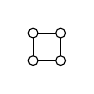
\begin{tikzpicture}[scale=0.35]
    \draw (0,0) -- (0,1);
    \draw (0,0) -- (1,0);
    \draw (1,1) -- (1,0);
    \draw (1,1) -- (0,1);

    \draw[fill=white](0,0) circle (5pt);
    \draw[fill=white](0,1) circle (5pt);
    \draw[fill=white](1,0) circle (5pt);
    \draw[fill=white](1,1) circle (5pt);
\end{tikzpicture} &\\
&3 && 0 && 2 && 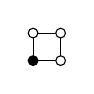
\begin{tikzpicture}[scale=0.35]
    \draw (0,0) -- (0,1);
    \draw (0,0) -- (1,0);
    \draw (1,1) -- (1,0);
    \draw (1,1) -- (0,1);

    \draw[fill=black](0,0) circle (5pt);
    \draw[fill=white](0,1) circle (5pt);
    \draw[fill=white](1,0) circle (5pt);
    \draw[fill=white](1,1) circle (5pt);
\end{tikzpicture}
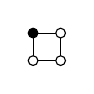
\begin{tikzpicture}[scale=0.35]
    \draw (0,0) -- (0,1);
    \draw (0,0) -- (1,0);
    \draw (1,1) -- (1,0);
    \draw (1,1) -- (0,1);

    \draw[fill=white](0,0) circle (5pt);
    \draw[fill=black](0,1) circle (5pt);
    \draw[fill=white](1,0) circle (5pt);
    \draw[fill=white](1,1) circle (5pt);
\end{tikzpicture}
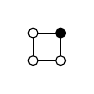
\begin{tikzpicture}[scale=0.35]
    \draw (0,0) -- (0,1);
    \draw (0,0) -- (1,0);
    \draw (1,1) -- (1,0);
    \draw (1,1) -- (0,1);

    \draw[fill=white](0,0) circle (5pt);
    \draw[fill=white](0,1) circle (5pt);
    \draw[fill=white](1,0) circle (5pt);
    \draw[fill=black](1,1) circle (5pt);
\end{tikzpicture}
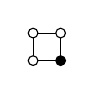
\begin{tikzpicture}[scale=0.35]
    \draw (0,0) -- (0,1);
    \draw (0,0) -- (1,0);
    \draw (1,1) -- (1,0);
    \draw (1,1) -- (0,1);

    \draw[fill=white](0,0) circle (5pt);
    \draw[fill=white](0,1) circle (5pt);
    \draw[fill=black](1,0) circle (5pt);
    \draw[fill=white](1,1) circle (5pt);
\end{tikzpicture}&\\
&2 && 0 && 0 && 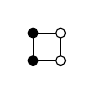
\begin{tikzpicture}[scale=0.35]
    \draw (0,0) -- (0,1);
    \draw (0,0) -- (1,0);
    \draw (1,1) -- (1,0);
    \draw (1,1) -- (0,1);

    \draw[fill=black](0,0) circle (5pt);
    \draw[fill=black](0,1) circle (5pt);
    \draw[fill=white](1,0) circle (5pt);
    \draw[fill=white](1,1) circle (5pt);
\end{tikzpicture}
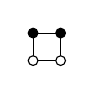
\begin{tikzpicture}[scale=0.35]
    \draw (0,0) -- (0,1);
    \draw (0,0) -- (1,0);
    \draw (1,1) -- (1,0);
    \draw (1,1) -- (0,1);

    \draw[fill=white](0,0) circle (5pt);
    \draw[fill=black](0,1) circle (5pt);
    \draw[fill=white](1,0) circle (5pt);
    \draw[fill=black](1,1) circle (5pt);
\end{tikzpicture}
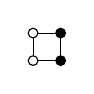
\begin{tikzpicture}[scale=0.35]
    \draw (0,0) -- (0,1);
    \draw (0,0) -- (1,0);
    \draw (1,1) -- (1,0);
    \draw (1,1) -- (0,1);

    \draw[fill=white](0,0) circle (5pt);
    \draw[fill=white](0,1) circle (5pt);
    \draw[fill=black](1,0) circle (5pt);
    \draw[fill=black](1,1) circle (5pt);
\end{tikzpicture}
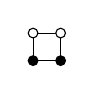
\begin{tikzpicture}[scale=0.35]
    \draw (0,0) -- (0,1);
    \draw (0,0) -- (1,0);
    \draw (1,1) -- (1,0);
    \draw (1,1) -- (0,1);

    \draw[fill=black](0,0) circle (5pt);
    \draw[fill=white](0,1) circle (5pt);
    \draw[fill=black](1,0) circle (5pt);
    \draw[fill=white](1,1) circle (5pt);
\end{tikzpicture}&\\
& 2 && 8J && 0 && 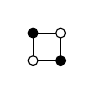
\begin{tikzpicture}[scale=0.35]
    \draw (0,0) -- (0,1);
    \draw (0,0) -- (1,0);
    \draw (1,1) -- (1,0);
    \draw (1,1) -- (0,1);

    \draw[fill=white](0,0) circle (5pt);
    \draw[fill=black](0,1) circle (5pt);
    \draw[fill=black](1,0) circle (5pt);
    \draw[fill=white](1,1) circle (5pt);
\end{tikzpicture}
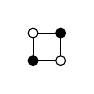
\begin{tikzpicture}[scale=0.35]
    \draw (0,0) -- (0,1);
    \draw (0,0) -- (1,0);
    \draw (1,1) -- (1,0);
    \draw (1,1) -- (0,1);

    \draw[fill=black](0,0) circle (5pt);
    \draw[fill=white](0,1) circle (5pt);
    \draw[fill=white](1,0) circle (5pt);
    \draw[fill=black](1,1) circle (5pt);
\end{tikzpicture}&\\
& 1 && 0 && -2 && 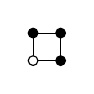
\begin{tikzpicture}[scale=0.35]
    \draw (0,0) -- (0,1);
    \draw (0,0) -- (1,0);
    \draw (1,1) -- (1,0);
    \draw (1,1) -- (0,1);

    \draw[fill=white](0,0) circle (5pt);
    \draw[fill=black](0,1) circle (5pt);
    \draw[fill=black](1,0) circle (5pt);
    \draw[fill=black](1,1) circle (5pt);
\end{tikzpicture}
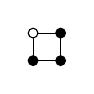
\begin{tikzpicture}[scale=0.35]
    \draw (0,0) -- (0,1);
    \draw (0,0) -- (1,0);
    \draw (1,1) -- (1,0);
    \draw (1,1) -- (0,1);

    \draw[fill=black](0,0) circle (5pt);
    \draw[fill=white](0,1) circle (5pt);
    \draw[fill=black](1,0) circle (5pt);
    \draw[fill=black](1,1) circle (5pt);
\end{tikzpicture}
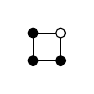
\begin{tikzpicture}[scale=0.35]
    \draw (0,0) -- (0,1);
    \draw (0,0) -- (1,0);
    \draw (1,1) -- (1,0);
    \draw (1,1) -- (0,1);

    \draw[fill=black](0,0) circle (5pt);
    \draw[fill=black](0,1) circle (5pt);
    \draw[fill=black](1,0) circle (5pt);
    \draw[fill=white](1,1) circle (5pt);
\end{tikzpicture}
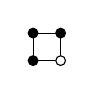
\begin{tikzpicture}[scale=0.35]
    \draw (0,0) -- (0,1);
    \draw (0,0) -- (1,0);
    \draw (1,1) -- (1,0);
    \draw (1,1) -- (0,1);

    \draw[fill=black](0,0) circle (5pt);
    \draw[fill=black](0,1) circle (5pt);
    \draw[fill=white](1,0) circle (5pt);
    \draw[fill=black](1,1) circle (5pt);
\end{tikzpicture}&\\
& 0 && -8J && -4 && 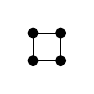
\begin{tikzpicture}[scale=0.35]
    \draw (0,0) -- (0,1);
    \draw (0,0) -- (1,0);
    \draw (1,1) -- (1,0);
    \draw (1,1) -- (0,1);

    \draw[fill=black](0,0) circle (5pt);
    \draw[fill=black](0,1) circle (5pt);
    \draw[fill=black](1,0) circle (5pt);
    \draw[fill=black](1,1) circle (5pt);
\end{tikzpicture}&\\
\hline
\end{tabularx}
\end{table}

Inserting the values from table \ref{tab:states} into equation \ref{eq:partition} gives the following partition function

\begin{flalign}
\nonumber Z &= 1e^{-\beta(-8J)} + 4 + 4 + 2e^{-\beta(8J)} + 4 + 1e^{-\beta(-8J)} \\
\nonumber   &= 2e^{8\beta J} + 2e^{-8\beta J} + 12 \\
            &= 4\cosh{8\beta J} + 12 
\label{eq:2by2_partition}
\end{flalign}

Inserting the values from table \ref{tab:states} into equation \ref{eq:mean_E} and computing the expected energy per spin gives:

\begin{flalign}
\nonumber \left\langle \frac{E}{N} \right\rangle &= \frac{-8Je^{-\beta(-8J)} + 2\cdot 8Je^{-\beta 8J} + (-8J)e^{-\beta(-8J)}}{ZN}  \\
\nonumber &= \frac{-16Je^{8\beta J} + 16Je^{-8\beta J}}{ZN} \\
&= \frac{-32J\sinh{8\beta J}}{ZN}
\label{eq:2by2_energy}
\end{flalign}

Inserting the values from table \ref{tab:states} into equation \ref{eq:mean_M} the expectation value of magnetization per spin becomes

\begin{flalign}
\nonumber \left\langle \frac{M}{N} \right\rangle &= \frac{4e^{-\beta(-8J)} + 4\cdot 2 + 4\cdot (-2) + (-4)e^{-\beta(-8J)}}{ZN} \\
 &= 0
\label{eq:2by2_magnetization}
\end{flalign}

\noindent and the expectation value of the absolute magnetization per spin becomes
\begin{flalign}
\nonumber \left\langle \frac{|\mathcal{M}|}{N} \right\rangle &= \frac{|4|e^{-\beta(-8J)} + 4|2| + 4|-2| + |-4|e^{-\beta(-8J)}}{ZN} \\
&= \frac{8e^{8\beta J} + 16}{ZN} 
\label{eq:2by2_abs_magnetization}
\end{flalign}

The second moment needed to compute the variance of the energy in equation \ref{eq:sigma_E} is

\begin{flalign}
\nonumber  \left\langle \left(\frac{E}{N}\right)^2\right\rangle &= \frac{(-8J)^2e^{-\beta(-8J)} + 2\cdot (8J)^2e^{-\beta 8J} + (-8J)^2e^{-\beta(-8J)}}{ZN^2}  \\
\nonumber &= \frac{64J^2e^{8\beta J} + 128J^2e^{-8\beta J} + 64J^2e^{8\beta J}}{ZN^2} \\
&= \frac{256J^2\cosh{8\beta J}}{ZN^2}
\end{flalign}

\noindent which gives the specific heat (per spin) as

\begin{flalign}
C_V &= \frac{\left\langle \left(\frac{E}{N}\right)^2\right\rangle - \left\langle \frac{E}{N}\right\rangle^2}{k_BT^2} 
\label{eq:2by2_specific_heat}
\end{flalign}

The second moment needed to compute the variance of the absolute magnetization in equation \ref{eq:sigma_M} is 

\begin{flalign}
\nonumber \left\langle \left(\frac{\mathcal{M}}{N}\right)^2 \right\rangle &= \frac{4^2e^{-\beta(-8J)} + 4\cdot 2^2 + 4\cdot (-2)^2 + (-4)^2e^{-\beta(-8J)}}{ZN^2} \\
\nonumber &= \frac{16e^{8\beta J} + 16  + 16 + 16e^{8\beta J}}{ZN^2}  \\
&= \frac{32e^{8\beta J} + 32}{ZN^2}
\end{flalign}

\noindent which finally gives the susceptibility (per spin) as 

\begin{flalign}
\chi = \frac{\left\langle \left(\frac{|\mathcal{M}|}{N}\right)^2\right\rangle - \left\langle \left(\frac{|\mathcal{M}|}{N}\right)\right\rangle^2}{k_BT}
\label{eq:2by2_susceptibility}
\end{flalign}

\FloatBarrier
\subsection{Metropolis algorithm for the Ising Model}
Obviously, calculating the expectation values for larger grids quickly becomes unfeasible and eventually impossible as the number of micro states grows exponentially. The Metropolis algorithm is a popular numerical recipe that can simulate the evolution of the micro states as time progresses. The algorithm should eventually reach a steady state and the various expectation values can be obtained. A quick summary of the derivation of the metropolis algorithm described in \cite{lectures} follows.

Given a discrete normalized probability distribution function, $\omega_i(t)$, that represents the probability of the system being in state $i$ at time $t$. For the Ising model this probability is given in equation \ref{eq:boltzmann}. The probability of being in state $i$ after a time step $\Delta t$ is given by

\begin{equation}
\omega_i(t+\Delta t) = \sum\limits_{j=1}^M W(j\rightarrow i) \omega_j(t) 
\end{equation}
where $W(j\rightarrow i)$ is a normalized probability of moving from state $j$ to state $i$, also referred to a the transition probability. $M$ is the total number of possible micro states. However, the transition probability is not known and computing a sum over all micro states is not feasible. Defining two new normalized probabilities, $T$ and $A$, where $T_{j\rightarrow i}$ represents the probability of suggesting a transition from state $i$ to state $j$ and $A_{j\rightarrow i}$ represent the probability of accepting the suggested transition. The probability of being in state $\omega_i$ after a time step is then the sum of the probability of accepting a suggested move to state $i$ and already being in state $i$ and rejecting a suggested move to another state. This can be written as

\begin{equation}
\omega_i(t+\Delta t) = \sum\limits_{j=1}^M (\omega_j(t)T_{j\rightarrow i}A_{j\rightarrow i} + \omega_i(t)T_{i\rightarrow j}(1 - A_{i\rightarrow j}))
\label{eq:transition}
\end{equation}

By exploiting the fact that $\sum\limits_j T_{i\rightarrow j} = 1$, equation \ref{eq:transition} can be rewritten as

\begin{equation}
\omega_i(t+\Delta t) - \omega_i(t) = \sum\limits_{j=1}^M (\omega_j(t)T_{j\rightarrow i}A_{j\rightarrow i} - \omega_i(t)T_{i\rightarrow j}A_{i\rightarrow j})
\end{equation}

When a steady state has been reached $\omega_i(t+\Delta t) - \omega_i(t) = 0$ which leads to the equilibrium constraint 

\begin{equation}
\sum\limits_{j=1}^M \omega_jT_{j\rightarrow i}A_{j\rightarrow i} = \sum\limits_{j=1}^M \omega_iT_{i\rightarrow j}A_{i\rightarrow j}
\end{equation}
Where the time $t$ is now ignored since equilibrium has been reached. This constraint may lead to cyclic solution, as stated in \cite{lectures} and an even stronger constraint is needed. This constraint is called detailed balance an is given by 

\begin{equation}
\omega_jT_{j\rightarrow i}A_{j\rightarrow i} = \omega_iT_{i\rightarrow j}A_{i\rightarrow j}
\end{equation}
which can be rewritten as 

\begin{equation}
\frac{\omega_i}{\omega_j} = \frac{T_{j\rightarrow i}A_{j\rightarrow i}}{T_{i\rightarrow j}A_{i\rightarrow j}}
\end{equation}
With no information about which moves are more likely, suggesting a move should have the same probability for all moves, meaning $T_{j\rightarrow i}=T_{i\rightarrow j}$. Exploiting this fact and inserting equation \ref{eq:boltzmann} for $\omega$ gives:

\begin{equation}
\frac{A_{j\rightarrow i}}{A_{i\rightarrow j}} = \frac{e^{-\beta E_i}}{e^{-\beta E_j}} = e^{-\beta(E_i - E_j)} = e^{-\beta \Delta E}
\end{equation}

The individual probabilities $0 \leq A_{j\rightarrow i} \leq 1$ and $0 \leq A_{i\rightarrow j} \leq 1$ are unknown, but their ratio is known. By fixing $A_{j\rightarrow i}=1$ when $E_i < E_j$ and fixing $A_{i\rightarrow j}=1$ when $E_i \geq E_j$, the probability of accepting the new state $i$ is then

\begin{equation}
A_{j\rightarrow i} = \min(1, e^{-\beta \Delta E})
\end{equation}
The Metropolis algorithm can be summarized as follows:

\fbox{\parbox{\textwidth}{
\begin{itemize}
\item Initialize the lattice to the desired starting state
\item For each Monte Carlo cycle
\begin{itemize}
\item For each spin in the lattice
\begin{itemize}
\item Select a random spin (using a uniform distribution)
\item Calculate the energy difference $\Delta E$ caused by flipping that spin
\item Select a random number $r$ between 0 and 1 from a uniform distribution
\item Accept the spin flip if $r \leq e^{-\beta\Delta E}$
\end{itemize}
\end{itemize}
\end{itemize}}} \\ 

\noindent The expectation values can then be approximated with 

\begin{equation}
\langle X \rangle = \frac{1}{m}\sum\limits_{i=1}^{m} X_{i}
\end{equation}
where the sum is over all cycles ${m}$ and $X_i$ is a parameter, for instance the system's energy, after cycle $i$. 

Since the energy in the Ising model only depends on the nearest neighbors, there is a limited set of possible changes to the energy when flipping one spin. By inserting equation \ref{eq:energy} the energy difference is given by

\begin{equation}
\Delta E = E_i - E_j = J\sum\limits_{<kl>}^N s_{k_j} s_{l_j} - J\sum\limits_{<kl>}^N s_{k_i} s_{l_i}
\end{equation}

Only flipping one spin at the time, say $s_l$, means that $s_{k_j}=s_{k_i}=s_k$. The energy difference then becomes

\begin{equation}
\Delta E = J\sum\limits_{<kl>}^N s_k(s_{l_j} - s_{l_i})
\end{equation}

The difference $s_{l_j} - s_{l_i}$ can only take on two possible values. If $s_{l_j}=1$ the difference becomes $2$ and if $s_{l_j}=-1$ the difference becomes $-2$. This is also the difference in the magnetization caused by the spin flip, only with opposite sign. The energy difference can then be simplified to

\begin{equation}
\Delta E = 2Js_{l_j} \sum\limits_{<k>} s_k
\end{equation}

where the sum is over the neighbors $<k>$ of spin $s_l$. This expression can only take on 5 specific values, summarized in table \ref{tab:deltaE}. 

\begin{table}
\centering
\caption{Difference in energy after flipping one spin}
\label{tab:deltaE}
\begin{tabular}{m{0.25\textwidth} m{0.30\textwidth} m{0.25\textwidth} m{0.20\textwidth}} 
\hline
Neighbors & $E_j$ & $E_i$ & $\Delta E$\\
\hline\hline
4 with same spin & 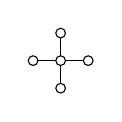
\begin{tikzpicture}[scale=0.35]
    \draw (0,0) -- (0,1);
    \draw (0,0) -- (1,0);
    \draw (0,0) -- (-1,0);
    \draw (0,0) -- (0,-1);

    \draw[fill=white](0,0) circle (5pt);
    \draw[fill=white](-1,0) circle (5pt);
    \draw[fill=white](0,1) circle (5pt);
    \draw[fill=white](1,0) circle (5pt);
    \draw[fill=white](0,-1) circle (5pt);
\end{tikzpicture} & 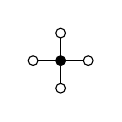
\begin{tikzpicture}[scale=0.35]
    \draw (0,0) -- (0,1);
    \draw (0,0) -- (1,0);
    \draw (0,0) -- (-1,0);
    \draw (0,0) -- (0,-1);

    \draw[fill=black](0,0) circle (5pt);
    \draw[fill=white](-1,0) circle (5pt);
    \draw[fill=white](0,1) circle (5pt);
    \draw[fill=white](1,0) circle (5pt);
    \draw[fill=white](0,-1) circle (5pt);
\end{tikzpicture} & 8J \\
3 with same spin & 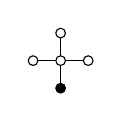
\begin{tikzpicture}[scale=0.35]
    \draw (0,0) -- (0,1);
    \draw (0,0) -- (1,0);
    \draw (0,0) -- (-1,0);
    \draw (0,0) -- (0,-1);

    \draw[fill=white](0,0) circle (5pt);
    \draw[fill=white](-1,0) circle (5pt);
    \draw[fill=white](0,1) circle (5pt);
    \draw[fill=white](1,0) circle (5pt);
    \draw[fill=black](0,-1) circle (5pt);
\end{tikzpicture} & 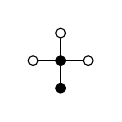
\begin{tikzpicture}[scale=0.35]
    \draw (0,0) -- (0,1);
    \draw (0,0) -- (1,0);
    \draw (0,0) -- (-1,0);
    \draw (0,0) -- (0,-1);

    \draw[fill=black](0,0) circle (5pt);
    \draw[fill=white](-1,0) circle (5pt);
    \draw[fill=white](0,1) circle (5pt);
    \draw[fill=white](1,0) circle (5pt);
    \draw[fill=black](0,-1) circle (5pt);
\end{tikzpicture} & 4J \\
2 with same spin & 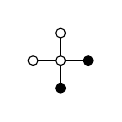
\begin{tikzpicture}[scale=0.35]
    \draw (0,0) -- (0,1);
    \draw (0,0) -- (1,0);
    \draw (0,0) -- (-1,0);
    \draw (0,0) -- (0,-1);

    \draw[fill=white](0,0) circle (5pt);
    \draw[fill=white](-1,0) circle (5pt);
    \draw[fill=white](0,1) circle (5pt);
    \draw[fill=black](1,0) circle (5pt);
    \draw[fill=black](0,-1) circle (5pt);
\end{tikzpicture} & 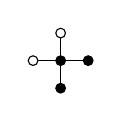
\begin{tikzpicture}[scale=0.35]
    \draw (0,0) -- (0,1);
    \draw (0,0) -- (1,0);
    \draw (0,0) -- (-1,0);
    \draw (0,0) -- (0,-1);

    \draw[fill=black](0,0) circle (5pt);
    \draw[fill=white](-1,0) circle (5pt);
    \draw[fill=white](0,1) circle (5pt);
    \draw[fill=black](1,0) circle (5pt);
    \draw[fill=black](0,-1) circle (5pt);
\end{tikzpicture} &  0 \\
1 with same spin & 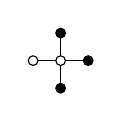
\begin{tikzpicture}[scale=0.35]
    \draw (0,0) -- (0,1);
    \draw (0,0) -- (1,0);
    \draw (0,0) -- (-1,0);
    \draw (0,0) -- (0,-1);

    \draw[fill=white](0,0) circle (5pt);
    \draw[fill=white](-1,0) circle (5pt);
    \draw[fill=black](0,1) circle (5pt);
    \draw[fill=black](1,0) circle (5pt);
    \draw[fill=black](0,-1) circle (5pt);
\end{tikzpicture} & 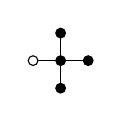
\begin{tikzpicture}[scale=0.35]
    \draw (0,0) -- (0,1);
    \draw (0,0) -- (1,0);
    \draw (0,0) -- (-1,0);
    \draw (0,0) -- (0,-1);

    \draw[fill=black](0,0) circle (5pt);
    \draw[fill=white](-1,0) circle (5pt);
    \draw[fill=black](0,1) circle (5pt);
    \draw[fill=black](1,0) circle (5pt);
    \draw[fill=black](0,-1) circle (5pt);
\end{tikzpicture} &-4J \\
0 with same spin & 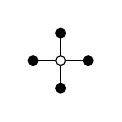
\begin{tikzpicture}[scale=0.35]
    \draw (0,0) -- (0,1);
    \draw (0,0) -- (1,0);
    \draw (0,0) -- (-1,0);
    \draw (0,0) -- (0,-1);

    \draw[fill=white](0,0) circle (5pt);
    \draw[fill=black](-1,0) circle (5pt);
    \draw[fill=black](0,1) circle (5pt);
    \draw[fill=black](1,0) circle (5pt);
    \draw[fill=black](0,-1) circle (5pt);
\end{tikzpicture} & 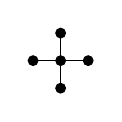
\begin{tikzpicture}[scale=0.35]
    \draw (0,0) -- (0,1);
    \draw (0,0) -- (1,0);
    \draw (0,0) -- (-1,0);
    \draw (0,0) -- (0,-1);

    \draw[fill=black](0,0) circle (5pt);
    \draw[fill=black](-1,0) circle (5pt);
    \draw[fill=black](0,1) circle (5pt);
    \draw[fill=black](1,0) circle (5pt);
    \draw[fill=black](0,-1) circle (5pt);
\end{tikzpicture} &-8J \\
\hline
\end{tabular}
\end{table}

\FloatBarrier
\section{Results}
\label{sec:results}
The source code for this project is located at http://github.com/annsilje/fys3150. For all the simulations the Boltzmann constant $k_B=1$ and the coupling constant $J=1$. First, a simple $2\times 2$ lattice is tested to verify that the numerical solution agrees with the analytical solution in section \ref{subsec:2by2}. Then a larger lattice ($20 \times 20$) is tested to investigate the behavior of the expectation values during the Monte Carlo cycles. Finally, multiple lattices are simulated where the temperature is gradually increased towards and beyond the critical temperature. 

\FloatBarrier
\subsection{2x2 lattice}
Setting the temperature $T=1.0$, the analytical values for the $2\times 2$ lattice is calculated using equations \ref{eq:2by2_partition}, \ref{eq:2by2_energy}, \ref{eq:2by2_magnetization}, \ref{eq:2by2_abs_magnetization}, \ref{eq:2by2_specific_heat} and \ref{eq:2by2_susceptibility} and compared to the values computed with the Metropolis algorithm. The results are summarized in table \ref{tab:analytical_vs_numerical}. The numerical results are in good agreement with the analytical results. One million Monte Carlo cycles seems to be sufficient to get decent numerical results and maybe even less for this small grid. 

\begin{table}
\centering
\caption{Numerical vs analytical results for a 2x2 lattice for increasing number of Monte Carlo cycles. The temperature is set to 1.0 and the lattice is initialized to a random micro state. }
\label{tab:analytical_vs_numerical}
\begin{tabularx}{\textwidth}{r r r r r r}
\hline
Cycles & $\langle E/N \rangle$ & $\langle M/N \rangle$& $\langle |M|/N \rangle$ & $C_V/N$ & $\chi/N$  \\
\hline\hline
$10^3$ & -1.996000 &  0.881500 & 0.999500 & 0.0079840 & -0.0002502\\
$10^4$ & -1.996200 & -0.171950 & 0.998850 & 0.0075855 &  0.0007736\\
$10^5$ & -1.996020 &  0.171705 & 0.998715 & 0.0079441 &  0.0009308\\
$10^6$ & -1.995898 & -0.086173 & 0.998611 & 0.0081871 &  0.0010553\\ 
$10^7$ & -1.995981 & -0.008413 & 0.998662 & 0.0080222 &  0.0009996\\
$10^8$ & -1.995991 & -0.001382 & 0.998663 & 0.0080016 &  0.0010005\\
\hline \hline
Analytical & -1.995982 & 0 & 0.998661  & 0.0080206 & 0.0010027 \\
\hline
\end{tabularx}
\end{table}

\FloatBarrier
\subsection{20x20 lattice}
With a $20\times 20$ lattice the number of Monte Carlo cycles needed to reach equilibrium is studied more carefully. Figure \ref{fig:no_cycles} shows how the number of accepted spin flips, mean energy and mean (absolute) magnetization evolves for each Monte Carlo cycle. 

First of all the percentage of accepted spin flips seems to be highly correlated with the mean energy since the two plots have a very similar shape for both $T=1.0$ and $T=2.4$. This seem natural since a spin flip is accepted based on the change in energy. For $T=1.0$ only a very small percentage ($\sim 0.07\%$) of spin flips are accepted when the solution has stabilized. For $T=2.4$ this percentage is much higher ($\sim 27\%$). The starting condition influences how fast the solution stabilizes and it can be seen most clearly for $T=1.0$. A random starting configuration is pretty far from the steady state for low temperatures and the solution requires more cycles to stabilize than the starting condition with all the spins up. For $T=2.4$ more Monte Carlo cycles is needed to stabilize the solution and it is not entirely clear whether $10^6$ cycles is enough. 

\begin{figure}
\centering
\subcaptionbox{T=1.0}[0.48\textwidth]{%
    \includegraphics[width=0.48\linewidth]{fig/{20x20_accepted1.0}.pdf}
\label{subfig:accepted10}
}
\subcaptionbox{T=2.4}[0.48\textwidth]{%
    \includegraphics[width=0.48\linewidth]{fig/{20x20_accepted2.4}.pdf}
    \label{subfig:accepted24}
}
\subcaptionbox{T=1.0}[0.48\textwidth]{%
    \includegraphics[width=0.48\linewidth]{fig/{20x20_energy1.0}.pdf}
\label{subfig:energy10}
}
\subcaptionbox{T=2.4}[0.48\textwidth]{%
    \includegraphics[width=0.48\linewidth]{fig/{20x20_energy2.4}.pdf}
\label{subfig:energy24}
}
\subcaptionbox{T=1.0}[0.48\textwidth]{%
    \includegraphics[width=0.48\linewidth]{fig/{20x20_abs_magnetization1.0}.pdf}
\label{subfig:magnetization10}
}
\subcaptionbox{T=2.4}[0.48\textwidth]{%
    \includegraphics[width=0.48\linewidth]{fig/{20x20_abs_magnetization2.4}.pdf}
\label{subfig:magnetization24}
}
\caption{Expectation values as a function of Monte Carlo cycles for different starting conditions and temperatures. The sampling rate is 100 cycles. (a) and (b) shows the percentage of accepted spin flips. (c) and (d) shows the mean energy and (e) and (f) shows the mean (absolute) magnetization.}
\label{fig:no_cycles}
\end{figure}

After the initial $10^6$ Monte Carlo cycles, another $10^4$ Monte Carlo cycles is run where the number of times a specific energy occurs is counted and then finally normalized. This should now represent an approximation to the probability distribution function $P(E)$ for the energy. The results are shown in figure \ref{fig:pdf}. 

For $T=2.4$ the plot resembles a normal distribution. For a perfect normal distribution the area under the distribution function and between the red vertical lines should be 68.2\% of the total area. For $T=1.0$, however, the system is limited by the minimum energy of -2J per spin and the sampling fails to produce a decent normal distribution and the minimal energy constitutes a relatively high peak in the probability distribution function.

\begin{figure}
\centering
\subcaptionbox{T=1.0}[0.48\textwidth]{
    \includegraphics[width=0.48\linewidth]{fig/{energy_pdf_temp1.0}.pdf}
\label{subfig:pdf10}
}
\subcaptionbox{T=2.4}[0.48\textwidth]{
    \includegraphics[width=0.48\linewidth]{fig/{energy_pdf_temp2.4}.pdf}
\label{subfig:pdf24}
}
\caption{Normalized occurrences of valid energy values during $10^4$ Monte Carlo cycles performed after equilibrium has been reached. The vertical red lines are one standard deviation from the mean value. (a) shows the energy occurrences with T=1.0 and (b) shows the energy occurrences with T=2.4.}
\label{fig:pdf}
\end{figure}

\FloatBarrier
\subsection{Parallelization}
Monte Carlo simulation usually requires a high number of samples and can become computationally heavy. It is therefore important to utilize some optimization and parallelization techniques to lower the execution time. By using the optimization flag \texttt{-O3} when compiling the compiler will try to optimize the code and how it is executed. This does not require any changes to the code, but the degree of optimization gained may depend on how the code is written. 

Parallelization, through the use of MPI (Message Passing Interface) for instance, requires changes to the code. The idea is to split the code into independent parts that can execute in parallel and communicate through a message interface. The Monte Carlo algorithm for the Ising Model can be parallelized by splitting the total number of cycles into $n$ parallel simulations. When a simulation is complete it needs to communicate the expectation values to the main process. For $10^6$ Monte Carlo cycles and using 4 processes each process then performs 250000 Monte Carlo cycles. All the processes start from the same initial conditions and needs to stabilize independently. Since the number of Monte Carlo cycles per process is reduced it becomes even more important to have a reasonable good starting condition. 

For a $30 \times 30$ lattice with $10^6$ Monte Carlo cycles the different speedup techniques are tested to verify that the execution time is reduced. The results are summarized in table \ref{tab:exec_times}. The results are slightly biased because without MPI the intermediate expectation values are written to file for every 100th cycle. With MPI no intermediate results are stored and the processes are not slowed down by writing to file. The results for MPI is also the average time spent per process, and the four processes completed approximately at the same time.

Regardless, the results clearly shows that both optimization and parallelization significantly improves execution times.

\begin{table}
\centering
\caption{Execution times for a $30\times 30$ lattice for $10^6$ Monte Carlo cycles with different optimization techniques}
\label{tab:exec_times}
\begin{tabularx}{\textwidth}{l r}
\hline
Optimization & Execution time (seconds) \\
\hline\hline
No flags and no MPI & 237 \\
-O3 flag and no MPI &  47 \\
-O3 flag and 4 MPI processes & 12 \\ 
\hline
\end{tabularx}
\end{table}


\FloatBarrier
\subsection{Critical temperature}

\begin{figure}
\centering
\subcaptionbox{Mean energy per spin\label{subfig:mean_energy}}[0.48\textwidth]{%
    \includegraphics[width=0.48\linewidth]{fig/mean_energy.pdf}
}
\subcaptionbox{Mean magnetization per spin\label{subfig:mean_magnetization}}[0.48\textwidth]{%
    \includegraphics[width=0.48\linewidth]{fig/mean_abs_magnetization.pdf}
}
\subcaptionbox{Specific heat per spin\label{subfig:heat_capacity}}[0.48\textwidth]{%
    \includegraphics[width=0.48\linewidth]{fig/heat_capacity.pdf}
}
\subcaptionbox{Susceptibility per spin\label{subfig:susceptibility}}[0.48\textwidth]{%
    \includegraphics[width=0.48\linewidth]{fig/susceptibility.pdf}
}
\caption{Monte Carlo simulations with increasing temperatures for different lattice sizes. (a) shows the mean energy per spin. (b) shows the mean absolute magnetization per spin. (c) shows the specific heat per spin and (d) shows the susceptibility per spin.}
\label{fig:temp_simulation}
\end{figure}


By running a full Monte Carlo simulation for a range of temperatures the behavior close to the critical temperature can be studied. The temperature range used in these experiments is $[2.10, 2.35]$ with increments of $0.01$. The number of Monte Carlo cycles used is $n^6$. The first Monte Carlo simulation starts with a random spin configuration, but all subsequent simulation starts with the final configuration from the previous temperature. The experiment is run with four different lattice sizes, namely $40 \times 40$, $60 \times 60$, $100 \times 100$ and $140 \times 140$. Figure \ref{fig:temp_simulation} shows the expectation values for the energy and absolute magnetization as the temperature increases, as well as the specific heat and susceptibility. 

The energy is increasing for increasing temperatures, as might be expected. The four different lattices disagree slightly on the value of the energy near the critical temperature. The (absolute) magnetization, however, exhibits a clearer effect of the lattice size. When the temperature reaches the critical temperature the model predicts that the magnetization is lost and should then be zero. Figure \ref{subfig:mean_magnetization}, however, shows a leading tail of magnetization also above the critical temperature. This tail seem to become smaller for larger lattice sizes and might be an artefact of the approximation of an infinite lattice with a finite lattice or the boundary conditions.

Both the specific heat and the susceptibility is expected to diverge around the critical temperature. Figure \ref{subfig:heat_capacity} and \ref{subfig:susceptibility} both show a spike in the region around the critical temperature, but the exact position of this spike seem to depend on the lattice size. The spikes in the susceptibility is also a bit clearer and cover a larger temperature range. Therefore, this plot is used to estimate the critical temperature. 

For each lattice the critical temperature is approximated as the temperature at the maximum value occurring in the susceptibility. This gives $T_C(L=40)=2.32$, $T_C(L=60)=2.30$, $T_C(L=100)=2.29$ and $T_C(L=140)=2.28$. By subtracting equation \ref{eq:crit} for a lattice from equation \ref{eq:crit} for a different lattice, the unknown $T_C(L=\infty)$ disappears and the constant $a$ can be estimated. Doing this for all pairs of lattices and computing the average $a$ from all these pairs yield $a= 2.29$. Then, using this $a$, $T_C(L=\infty)$ is computed for all the lattices and again a simple average is computed. This yields $T_C(L=\infty)= 2.263832$. The theoretical critical temperature $T_C$ is approximately $2.269$ for $\nu=1$, according to \cite{onsager}. This shows that the first three digits are correct. But having only four data points to determine two constants yields very few degrees of freedom and a large uncertainty in the estimate. 




\FloatBarrier
\section{Conclusions}
\label{sec:conclusions}
Using the Monte Carlo algorithm for the Ising Model requires many Monte Carlo cycles. At least $10^6$ and preferably even more. With $10^6$ Monte Carlo cycles the critical temperature is correct with respect to the analytical solution up to 3 digits. This estimate can be improved by applying a proper estimation method that would also give the variance of the estimate. In addition, the temperature step size could be decreased, the number of Monte Carlo cycles could be increased and larger and more lattices could be tested. This would, however, also increase computation time significantly. This Monte Carlo simulation has also benefited greatly from using optimization and parallelization. 


\clearpage

\begin{thebibliography}{1}
\bibitem{lectures} Hjort-Jensen, M., 2015. Computational physics. Available at https://github.com/CompPhysics/ComputationalPhysics/
%\bibitem{physics} Young, Freedman, Sears and Zemansky's University Physics with Modern Physics, 11th edition, Addison-Wesley, 2004  
%@article{PhysRev.65.117,
%  title = {Crystal Statistics. I. A Two-Dimensional Model with an Order-Disorder Transition},
%  author = {Onsager, Lars},
%  journal = {Phys. Rev.},
%  volume = {65},
%  issue = {3-4},
%  pages = {117--149},
%  numpages = {0},
%  year = {1944},
%  month = {Feb},
%  publisher = {American Physical Society},
%  doi = {10.1103/PhysRev.65.117},
%  url = {http://link.aps.org/doi/10.1103/PhysRev.65.117}
%}
\bibitem{onsager} Onsager, Lars, Phys. Rev., \textbf{65}, 117--149, (1944)
\end{thebibliography}





\end{document}
